\section{Inserção}

\begin{frame}[fragile]{Inserção no início}

    \begin{itemize}
        \item A inserção no início (\code{c++}{push_front()}) de uma lista circular tem
            complexidade $O(1)$

        \item O primeiro passo da inserção é criar um novo nó

        \item Em seguida, deve ser preenchido o campo \code{c++}{info}

        \item O membro \code{c++}{prev} deve ser nulo

        \item O membro \code{c++}{next} deve apontar então para o primeiro elemento da lista
        (\code{c++}{head})

        \item O membro \code{c++}{head} deve apontar para o novo elemento

        \item Por fim, é preciso reestabelecer o invariante da lista circular: o campo
        \code{c}{next} de \code{c}{tail} tem que apontar para \code{c}{head} e o campo
        \code{c}{prev} de \code{c}{head} tem que apontar para \code{c}{tail}
    \end{itemize}

\end{frame}

\begin{frame}[fragile]{Visualização da inserção no início}

    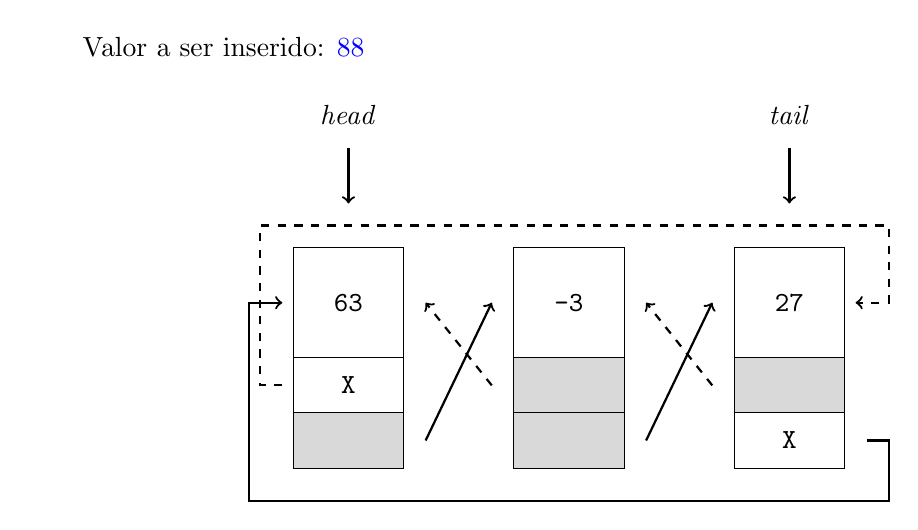
\begin{tikzpicture}[scale=1.4]
        \node[anchor=north west] at (0, 4) {Valor a ser inserido: \textcolor{blue}{88}};

        \node[anchor=center] at (2.5, 3.2) {\textit{head}};
        \draw[->,thick] (2.5, 2.9) -- (2.5, 2.4);

        \node[anchor=center] at (6.5, 3.2) {\textit{tail}};
        \draw[->,thick] (6.5, 2.9) -- (6.5, 2.4);

        \draw[opacity=0,->,thick] (7.2, 0.25) -- (7.4, 0.25) -- (7.4, -0.3) -- (-0.4, -0.3) -- (-0.4, 1.5) -- (-0.1, 1.5);
        \draw[opacity=0,->,thick,dashed] (-0.1, 0.75) -- (-0.3, 0.75) -- (-0.3, 2.2) -- (7.4, 2.2) -- (7.4, 1.5) -- (7.1, 1.5);

        \draw[->,thick] (7.2, 0.25) -- (7.4, 0.25) -- (7.4, -0.3) -- (1.6, -0.3) -- (1.6, 1.5) -- (1.9, 1.5);
        \draw[->,thick,dashed] (1.9, 0.75) -- (1.7, 0.75) -- (1.7, 2.2) -- (7.4, 2.2) -- (7.4, 1.5) -- (7.1, 1.5);

        \draw[opacity=0] (0,1) rectangle (1,2);


        \draw[fill=white] (2,1) rectangle (3,2);
        \draw (2,0.5) rectangle (3,1);
        \node at (2.5,0.75) { \textbf{\texttt{X}}};
        \draw[fill=gray!30] (2,0) rectangle (3,0.5);
        \node at (2.5,1.5) {\texttt{63}};

        \draw[->,thick] (3.2, 0.25) -- (3.8, 1.5);
        \draw[->,thick,dashed] (3.8, 0.75) -- (3.2, 1.5);

        \draw[fill=white] (4,1) rectangle (5,2);
        \draw[fill=gray!30] (4,0) rectangle (5,0.5);
        \draw[fill=gray!30] (4,0.5) rectangle (5,1);
        \node at (4.5,1.5) {\texttt{-3}};

        \draw[->,thick] (5.2, 0.25) -- (5.8, 1.5);
        \draw[->,thick,dashed] (5.8, 0.75) -- (5.2, 1.5);

        \draw[fill=white] (6,1) rectangle (7,2);
        \draw (6,0) rectangle (7,0.5);
        \draw[fill=gray!30] (6,0.5) rectangle (7,1);
        \node at (6.5,1.5) {\texttt{27}};
        \node at (6.5,0.25) {\textbf{\texttt{X}}};

    \end{tikzpicture}

\end{frame}

\begin{frame}[fragile]{Visualização da inserção no início}

    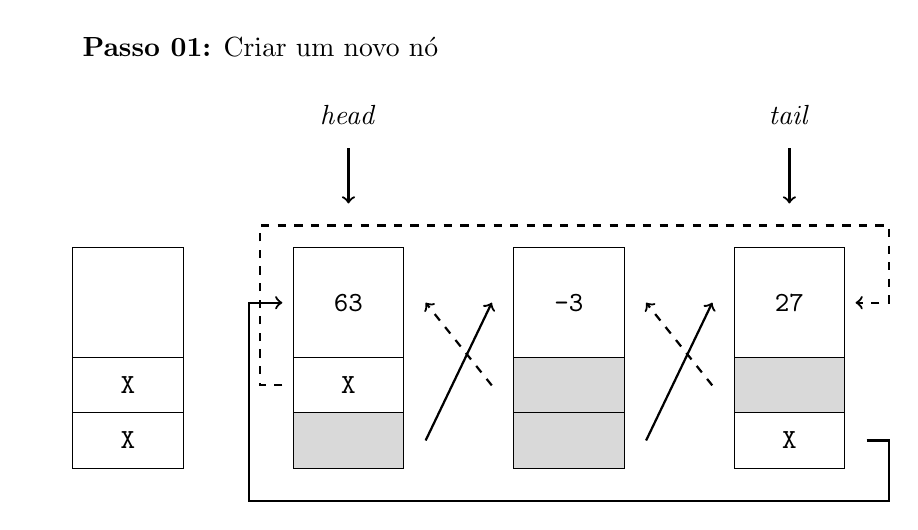
\begin{tikzpicture}[scale=1.4]
        \node[anchor=north west] at (0, 4) {\textbf{Passo 01:} Criar um novo nó};

        \node[anchor=center] at (2.5, 3.2) {\textit{head}};
        \draw[->,thick] (2.5, 2.9) -- (2.5, 2.4);

        \node[anchor=center] at (6.5, 3.2) {\textit{tail}};
        \draw[->,thick] (6.5, 2.9) -- (6.5, 2.4);

        \draw[opacity=0,->,thick] (7.2, 0.25) -- (7.4, 0.25) -- (7.4, -0.3) -- (-0.4, -0.3) -- (-0.4, 1.5) -- (-0.1, 1.5);
        \draw[opacity=0,->,thick,dashed] (-0.1, 0.75) -- (-0.3, 0.75) -- (-0.3, 2.2) -- (7.4, 2.2) -- (7.4, 1.5) -- (7.1, 1.5);

        \draw[->,thick] (7.2, 0.25) -- (7.4, 0.25) -- (7.4, -0.3) -- (1.6, -0.3) -- (1.6, 1.5) -- (1.9, 1.5);
        \draw[->,thick,dashed] (1.9, 0.75) -- (1.7, 0.75) -- (1.7, 2.2) -- (7.4, 2.2) -- (7.4, 1.5) -- (7.1, 1.5);

        \draw[fill=white] (0,1) rectangle (1,2);
        \draw (0,0.5) rectangle (1,1);
        \draw (0,0) rectangle (1,0.5);
        \node at (0.5,0.75) { \textbf{\texttt{X}}};
        \node at (0.5,0.25) { \textbf{\texttt{X}}};
        \node at (0.5,1.5) { \textcolor{white}{\texttt{63}}};

        \draw[fill=gray!30] (2,0) rectangle (3,0.5);
        \draw[fill=white] (2,1) rectangle (3,2);
        \draw (2,0.5) rectangle (3,1);
        \node at (2.5,0.75) { \textbf{\texttt{X}}};
        \draw[fill=gray!30] (2,0) rectangle (3,0.5);
        \node at (2.5,1.5) {\texttt{63}};

        \draw[->,thick] (3.2, 0.25) -- (3.8, 1.5);
        \draw[->,thick,dashed] (3.8, 0.75) -- (3.2, 1.5);

        \draw[fill=white] (4,1) rectangle (5,2);
        \draw[fill=gray!30] (4,0) rectangle (5,0.5);
        \draw[fill=gray!30] (4,0.5) rectangle (5,1);
        \node at (4.5,1.5) {\texttt{-3}};

        \draw[->,thick] (5.2, 0.25) -- (5.8, 1.5);
        \draw[->,thick,dashed] (5.8, 0.75) -- (5.2, 1.5);

        \draw[fill=white] (6,1) rectangle (7,2);
        \draw (6,0) rectangle (7,0.5);
        \draw[fill=gray!30] (6,0.5) rectangle (7,1);
        \node at (6.5,1.5) {\texttt{27}};
        \node at (6.5,0.25) {\textbf{\texttt{X}}};

    \end{tikzpicture}

\end{frame}

\begin{frame}[fragile]{Visualização da inserção no início}

    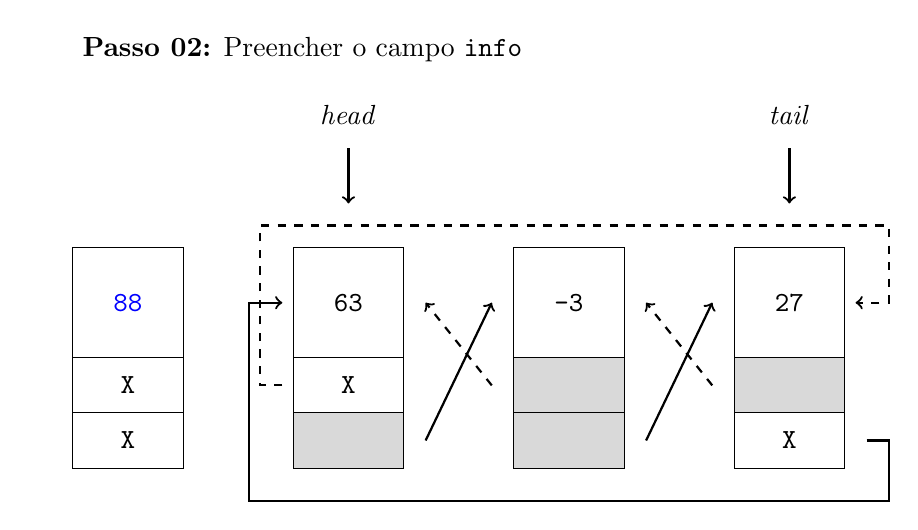
\begin{tikzpicture}[scale=1.4]
        \node[anchor=north west] at (0, 4) {\textbf{Passo 02:} Preencher o campo \texttt{info}};

        \node[anchor=center] at (2.5, 3.2) {\textit{head}};
        \draw[->,thick] (2.5, 2.9) -- (2.5, 2.4);

        \node[anchor=center] at (6.5, 3.2) {\textit{tail}};
        \draw[->,thick] (6.5, 2.9) -- (6.5, 2.4);

        \draw[opacity=0,->,thick] (7.2, 0.25) -- (7.4, 0.25) -- (7.4, -0.3) -- (-0.4, -0.3) -- (-0.4, 1.5) -- (-0.1, 1.5);
        \draw[opacity=0,->,thick,dashed] (-0.1, 0.75) -- (-0.3, 0.75) -- (-0.3, 2.2) -- (7.4, 2.2) -- (7.4, 1.5) -- (7.1, 1.5);

        \draw[->,thick] (7.2, 0.25) -- (7.4, 0.25) -- (7.4, -0.3) -- (1.6, -0.3) -- (1.6, 1.5) -- (1.9, 1.5);
        \draw[->,thick,dashed] (1.9, 0.75) -- (1.7, 0.75) -- (1.7, 2.2) -- (7.4, 2.2) -- (7.4, 1.5) -- (7.1, 1.5);

        \draw[fill=white] (0,1) rectangle (1,2);
        \draw (0,0.5) rectangle (1,1);
        \draw (0,0) rectangle (1,0.5);
        \node at (0.5,0.75) { \textbf{\texttt{X}}};
        \node at (0.5,0.25) { \textbf{\texttt{X}}};
        \node at (0.5,1.5) { \textcolor{blue}{\texttt{88}}};

        \draw[fill=gray!30] (2,0) rectangle (3,0.5);
        \draw[fill=white] (2,1) rectangle (3,2);
        \draw (2,0.5) rectangle (3,1);
        \node at (2.5,0.75) { \textbf{\texttt{X}}};
        \draw[fill=gray!30] (2,0) rectangle (3,0.5);
        \node at (2.5,1.5) {\texttt{63}};

        \draw[->,thick] (3.2, 0.25) -- (3.8, 1.5);
        \draw[->,thick,dashed] (3.8, 0.75) -- (3.2, 1.5);

        \draw[fill=white] (4,1) rectangle (5,2);
        \draw[fill=gray!30] (4,0) rectangle (5,0.5);
        \draw[fill=gray!30] (4,0.5) rectangle (5,1);
        \node at (4.5,1.5) {\texttt{-3}};

        \draw[->,thick] (5.2, 0.25) -- (5.8, 1.5);
        \draw[->,thick,dashed] (5.8, 0.75) -- (5.2, 1.5);

        \draw[fill=white] (6,1) rectangle (7,2);
        \draw (6,0) rectangle (7,0.5);
        \draw[fill=gray!30] (6,0.5) rectangle (7,1);
        \node at (6.5,1.5) {\texttt{27}};
        \node at (6.5,0.25) {\textbf{\texttt{X}}};

    \end{tikzpicture}

\end{frame}

\begin{frame}[fragile]{Visualização da inserção no início}

    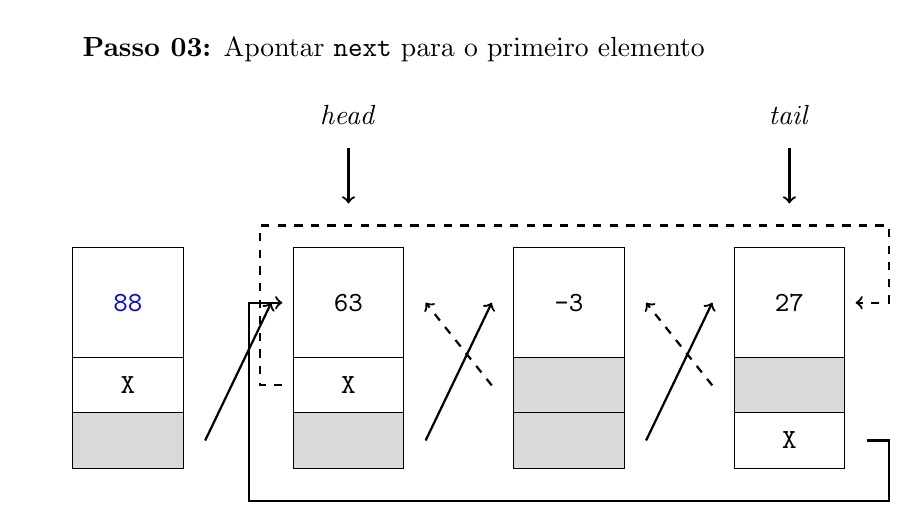
\begin{tikzpicture}[scale=1.4]
        \node[anchor=north west] at (0, 4) {\textbf{Passo 03:} Apontar \texttt{next} para o primeiro elemento};

        \node[anchor=center] at (2.5, 3.2) {\textit{head}};
        \draw[->,thick] (2.5, 2.9) -- (2.5, 2.4);

        \node[anchor=center] at (6.5, 3.2) {\textit{tail}};
        \draw[->,thick] (6.5, 2.9) -- (6.5, 2.4);

        \draw[opacity=0,->,thick] (7.2, 0.25) -- (7.4, 0.25) -- (7.4, -0.3) -- (-0.4, -0.3) -- (-0.4, 1.5) -- (-0.1, 1.5);
        \draw[opacity=0,->,thick,dashed] (-0.1, 0.75) -- (-0.3, 0.75) -- (-0.3, 2.2) -- (7.4, 2.2) -- (7.4, 1.5) -- (7.1, 1.5);

        \draw[->,thick] (7.2, 0.25) -- (7.4, 0.25) -- (7.4, -0.3) -- (1.6, -0.3) -- (1.6, 1.5) -- (1.9, 1.5);
        \draw[->,thick,dashed] (1.9, 0.75) -- (1.7, 0.75) -- (1.7, 2.2) -- (7.4, 2.2) -- (7.4, 1.5) -- (7.1, 1.5);

        \draw[fill=white] (0,1) rectangle (1,2);
        \draw (0,0.5) rectangle (1,1);
        \draw[fill=gray!30] (0,0) rectangle (1,0.5);
        \node at (0.5,0.75) { \textbf{\texttt{X}}};
        \node at (0.5,1.5) { \textcolor{blue}{\texttt{88}}};

        \draw[->,thick] (1.2, 0.25) -- (1.8, 1.5);

        \draw[fill=gray!30] (2,0) rectangle (3,0.5);
        \draw[fill=white] (2,1) rectangle (3,2);
        \draw (2,0.5) rectangle (3,1);
        \node at (2.5,0.75) { \textbf{\texttt{X}}};
        \draw[fill=gray!30] (2,0) rectangle (3,0.5);
        \node at (2.5,1.5) {\texttt{63}};

        \draw[->,thick] (3.2, 0.25) -- (3.8, 1.5);
        \draw[->,thick,dashed] (3.8, 0.75) -- (3.2, 1.5);

        \draw[fill=white] (4,1) rectangle (5,2);
        \draw[fill=gray!30] (4,0) rectangle (5,0.5);
        \draw[fill=gray!30] (4,0.5) rectangle (5,1);
        \node at (4.5,1.5) {\texttt{-3}};

        \draw[->,thick] (5.2, 0.25) -- (5.8, 1.5);
        \draw[->,thick,dashed] (5.8, 0.75) -- (5.2, 1.5);

        \draw[fill=white] (6,1) rectangle (7,2);
        \draw (6,0) rectangle (7,0.5);
        \draw[fill=gray!30] (6,0.5) rectangle (7,1);
        \node at (6.5,1.5) {\texttt{27}};
        \node at (6.5,0.25) {\textbf{\texttt{X}}};

    \end{tikzpicture}

\end{frame}

\begin{frame}[fragile]{Visualização da inserção no início}

    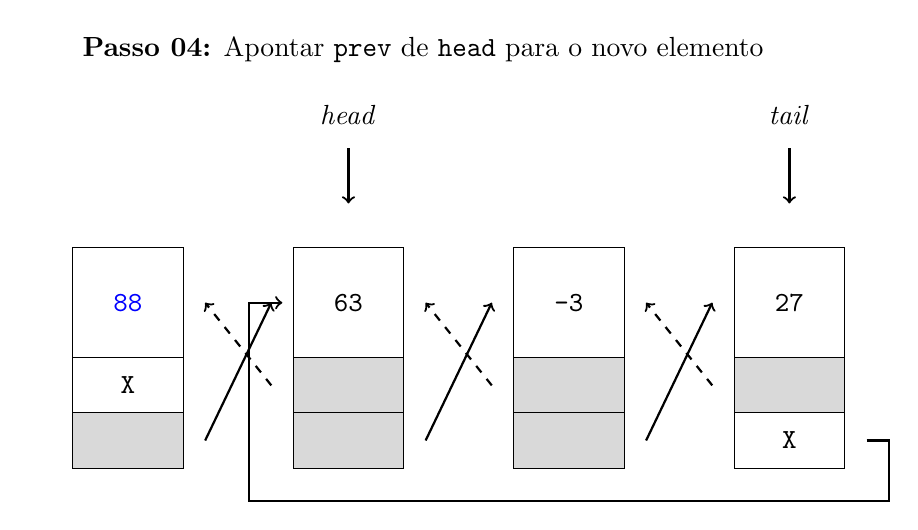
\begin{tikzpicture}[scale=1.4]
        \node[anchor=north west] at (0, 4) {\textbf{Passo 04:} Apontar \texttt{prev} de \texttt{head} para o novo elemento};

        \node[anchor=center] at (2.5, 3.2) {\textit{head}};
        \draw[->,thick] (2.5, 2.9) -- (2.5, 2.4);

        \node[anchor=center] at (6.5, 3.2) {\textit{tail}};
        \draw[->,thick] (6.5, 2.9) -- (6.5, 2.4);

        \draw[opacity=0,->,thick] (7.2, 0.25) -- (7.4, 0.25) -- (7.4, -0.3) -- (-0.4, -0.3) -- (-0.4, 1.5) -- (-0.1, 1.5);
        \draw[opacity=0,->,thick,dashed] (-0.1, 0.75) -- (-0.3, 0.75) -- (-0.3, 2.2) -- (7.4, 2.2) -- (7.4, 1.5) -- (7.1, 1.5);

        \draw[->,thick] (7.2, 0.25) -- (7.4, 0.25) -- (7.4, -0.3) -- (1.6, -0.3) -- (1.6, 1.5) -- (1.9, 1.5);

        \draw[fill=white] (0,1) rectangle (1,2);
        \draw (0,0.5) rectangle (1,1);
        \draw[fill=gray!30] (0,0) rectangle (1,0.5);
        \node at (0.5,0.75) { \textbf{\texttt{X}}};
        \node at (0.5,1.5) { \textcolor{blue}{\texttt{88}}};

        \draw[->,thick] (1.2, 0.25) -- (1.8, 1.5);
        \draw[->,thick,dashed] (1.8, 0.75) -- (1.2, 1.5);

        \draw[fill=gray!30] (2,0) rectangle (3,0.5);
        \draw[fill=white] (2,1) rectangle (3,2);
        \draw[fill=gray!30] (2,0.5) rectangle (3,1);
        \draw[fill=gray!30] (2,0) rectangle (3,0.5);
        \node at (2.5,1.5) {\texttt{63}};

        \draw[->,thick] (3.2, 0.25) -- (3.8, 1.5);
        \draw[->,thick,dashed] (3.8, 0.75) -- (3.2, 1.5);

        \draw[fill=white] (4,1) rectangle (5,2);
        \draw[fill=gray!30] (4,0) rectangle (5,0.5);
        \draw[fill=gray!30] (4,0.5) rectangle (5,1);
        \node at (4.5,1.5) {\texttt{-3}};

        \draw[->,thick] (5.2, 0.25) -- (5.8, 1.5);
        \draw[->,thick,dashed] (5.8, 0.75) -- (5.2, 1.5);

        \draw[fill=white] (6,1) rectangle (7,2);
        \draw (6,0) rectangle (7,0.5);
        \draw[fill=gray!30] (6,0.5) rectangle (7,1);
        \node at (6.5,1.5) {\texttt{27}};
        \node at (6.5,0.25) {\textbf{\texttt{X}}};

    \end{tikzpicture}

\end{frame}

\begin{frame}[fragile]{Visualização da inserção no início}

    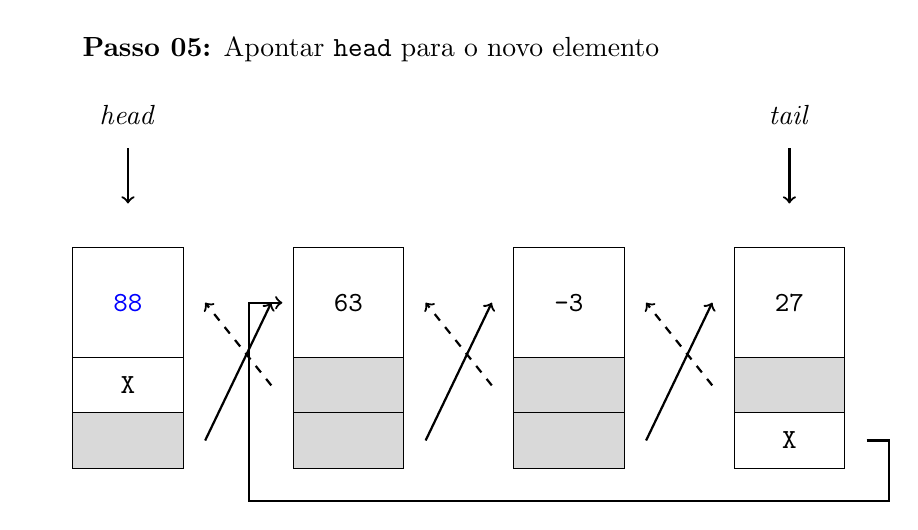
\begin{tikzpicture}[scale=1.4]
        \node[anchor=north west] at (0, 4) {\textbf{Passo 05:} Apontar \texttt{head} para o novo elemento};

        \node[anchor=center] at (0.5, 3.2) {\textit{head}};
        \draw[->,thick] (0.5, 2.9) -- (0.5, 2.4);

        \node[anchor=center] at (6.5, 3.2) {\textit{tail}};
        \draw[->,thick] (6.5, 2.9) -- (6.5, 2.4);

        \draw[opacity=0,->,thick] (7.2, 0.25) -- (7.4, 0.25) -- (7.4, -0.3) -- (-0.4, -0.3) -- (-0.4, 1.5) -- (-0.1, 1.5);
        \draw[opacity=0,->,thick,dashed] (-0.1, 0.75) -- (-0.3, 0.75) -- (-0.3, 2.2) -- (7.4, 2.2) -- (7.4, 1.5) -- (7.1, 1.5);

        \draw[->,thick] (7.2, 0.25) -- (7.4, 0.25) -- (7.4, -0.3) -- (1.6, -0.3) -- (1.6, 1.5) -- (1.9, 1.5);

        \draw[fill=white] (0,1) rectangle (1,2);
        \draw (0,0.5) rectangle (1,1);
        \draw[fill=gray!30] (0,0) rectangle (1,0.5);
        \node at (0.5,0.75) { \textbf{\texttt{X}}};
        \node at (0.5,1.5) { \textcolor{blue}{\texttt{88}}};

        \draw[->,thick] (1.2, 0.25) -- (1.8, 1.5);
        \draw[->,thick,dashed] (1.8, 0.75) -- (1.2, 1.5);

        \draw[fill=gray!30] (2,0) rectangle (3,0.5);
        \draw[fill=white] (2,1) rectangle (3,2);
        \draw[fill=gray!30] (2,0.5) rectangle (3,1);
        \draw[fill=gray!30] (2,0) rectangle (3,0.5);
        \node at (2.5,1.5) {\texttt{63}};

        \draw[->,thick] (3.2, 0.25) -- (3.8, 1.5);
        \draw[->,thick,dashed] (3.8, 0.75) -- (3.2, 1.5);

        \draw[fill=white] (4,1) rectangle (5,2);
        \draw[fill=gray!30] (4,0) rectangle (5,0.5);
        \draw[fill=gray!30] (4,0.5) rectangle (5,1);
        \node at (4.5,1.5) {\texttt{-3}};

        \draw[->,thick] (5.2, 0.25) -- (5.8, 1.5);
        \draw[->,thick,dashed] (5.8, 0.75) -- (5.2, 1.5);

        \draw[fill=white] (6,1) rectangle (7,2);
        \draw (6,0) rectangle (7,0.5);
        \draw[fill=gray!30] (6,0.5) rectangle (7,1);
        \node at (6.5,1.5) {\texttt{27}};
        \node at (6.5,0.25) {\textbf{\texttt{X}}};

    \end{tikzpicture}

\end{frame}

\begin{frame}[fragile]{Visualização da inserção no início}

    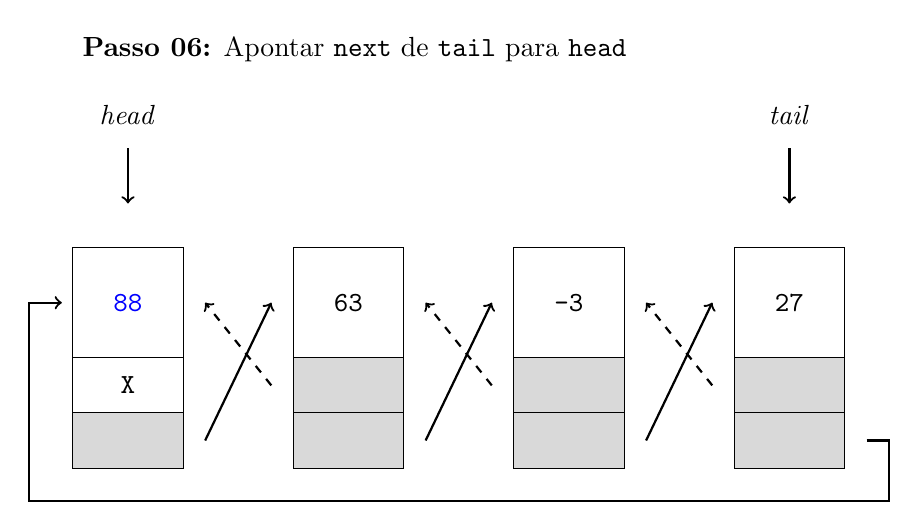
\begin{tikzpicture}[scale=1.4]
        \node[anchor=north west] at (0, 4) {\textbf{Passo 06:} Apontar \texttt{next} de \texttt{tail} para \texttt{head}};

        \node[anchor=center] at (0.5, 3.2) {\textit{head}};
        \draw[->,thick] (0.5, 2.9) -- (0.5, 2.4);

        \node[anchor=center] at (6.5, 3.2) {\textit{tail}};
        \draw[->,thick] (6.5, 2.9) -- (6.5, 2.4);

        \draw[opacity=1,->,thick] (7.2, 0.25) -- (7.4, 0.25) -- (7.4, -0.3) -- (-0.4, -0.3) -- (-0.4, 1.5) -- (-0.1, 1.5);
        \draw[opacity=0,->,thick,dashed] (-0.1, 0.75) -- (-0.3, 0.75) -- (-0.3, 2.2) -- (7.4, 2.2) -- (7.4, 1.5) -- (7.1, 1.5);


        \draw[fill=white] (0,1) rectangle (1,2);
        \draw (0,0.5) rectangle (1,1);
        \draw[fill=gray!30] (0,0) rectangle (1,0.5);
        \node at (0.5,0.75) { \textbf{\texttt{X}}};
        \node at (0.5,1.5) { \textcolor{blue}{\texttt{88}}};

        \draw[->,thick] (1.2, 0.25) -- (1.8, 1.5);
        \draw[->,thick,dashed] (1.8, 0.75) -- (1.2, 1.5);

        \draw[fill=gray!30] (2,0) rectangle (3,0.5);
        \draw[fill=white] (2,1) rectangle (3,2);
        \draw[fill=gray!30] (2,0.5) rectangle (3,1);
        \draw[fill=gray!30] (2,0) rectangle (3,0.5);
        \node at (2.5,1.5) {\texttt{63}};

        \draw[->,thick] (3.2, 0.25) -- (3.8, 1.5);
        \draw[->,thick,dashed] (3.8, 0.75) -- (3.2, 1.5);

        \draw[fill=white] (4,1) rectangle (5,2);
        \draw[fill=gray!30] (4,0) rectangle (5,0.5);
        \draw[fill=gray!30] (4,0.5) rectangle (5,1);
        \node at (4.5,1.5) {\texttt{-3}};

        \draw[->,thick] (5.2, 0.25) -- (5.8, 1.5);
        \draw[->,thick,dashed] (5.8, 0.75) -- (5.2, 1.5);

        \draw[fill=white] (6,1) rectangle (7,2);
        \draw[fill=gray!30] (6,0) rectangle (7,0.5);
        \draw[fill=gray!30] (6,0.5) rectangle (7,1);
        \node at (6.5,1.5) {\texttt{27}};

    \end{tikzpicture}

\end{frame}

\begin{frame}[fragile]{Visualização da inserção no início}

    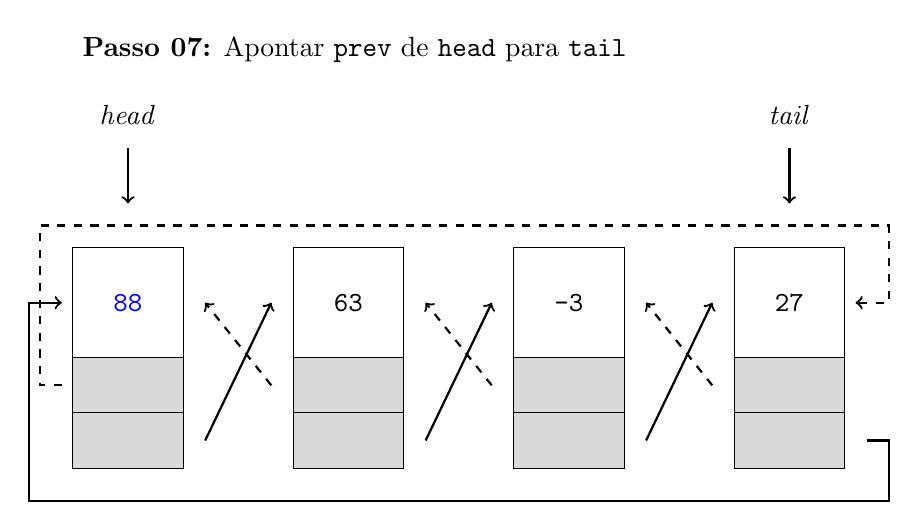
\begin{tikzpicture}[scale=1.4]
        \node[anchor=north west] at (0, 4) {\textbf{Passo 07:} Apontar \texttt{prev} de \texttt{head} para \texttt{tail}};

        \node[anchor=center] at (0.5, 3.2) {\textit{head}};
        \draw[->,thick] (0.5, 2.9) -- (0.5, 2.4);

        \node[anchor=center] at (6.5, 3.2) {\textit{tail}};
        \draw[->,thick] (6.5, 2.9) -- (6.5, 2.4);

        \draw[opacity=1,->,thick] (7.2, 0.25) -- (7.4, 0.25) -- (7.4, -0.3) -- (-0.4, -0.3) -- (-0.4, 1.5) -- (-0.1, 1.5);
        \draw[opacity=1,->,thick,dashed] (-0.1, 0.75) -- (-0.3, 0.75) -- (-0.3, 2.2) -- (7.4, 2.2) -- (7.4, 1.5) -- (7.1, 1.5);

        \draw[fill=white] (0,1) rectangle (1,2);
        \draw[fill=gray!30] (0,0.5) rectangle (1,1);
        \draw[fill=gray!30] (0,0) rectangle (1,0.5);
        \node at (0.5,1.5) { \textcolor{blue}{\texttt{88}}};

        \draw[->,thick] (1.2, 0.25) -- (1.8, 1.5);
        \draw[->,thick,dashed] (1.8, 0.75) -- (1.2, 1.5);

        \draw[fill=gray!30] (2,0) rectangle (3,0.5);
        \draw[fill=white] (2,1) rectangle (3,2);
        \draw[fill=gray!30] (2,0.5) rectangle (3,1);
        \draw[fill=gray!30] (2,0) rectangle (3,0.5);
        \node at (2.5,1.5) {\texttt{63}};

        \draw[->,thick] (3.2, 0.25) -- (3.8, 1.5);
        \draw[->,thick,dashed] (3.8, 0.75) -- (3.2, 1.5);

        \draw[fill=white] (4,1) rectangle (5,2);
        \draw[fill=gray!30] (4,0) rectangle (5,0.5);
        \draw[fill=gray!30] (4,0.5) rectangle (5,1);
        \node at (4.5,1.5) {\texttt{-3}};

        \draw[->,thick] (5.2, 0.25) -- (5.8, 1.5);
        \draw[->,thick,dashed] (5.8, 0.75) -- (5.2, 1.5);

        \draw[fill=white] (6,1) rectangle (7,2);
        \draw[fill=gray!30] (6,0) rectangle (7,0.5);
        \draw[fill=gray!30] (6,0.5) rectangle (7,1);
        \node at (6.5,1.5) {\texttt{27}};

    \end{tikzpicture}

\end{frame}



\begin{frame}[fragile]{Implementação da inserção no início}
    \inputsnippet{c++}{129}{140}{circular_list.h}
\end{frame}

\begin{frame}[fragile]{Inserção no final}

    \begin{itemize}
        \item A inserção no final (\code{c++}{push_back()}) de uma lista circular tem
            complexidade $O(1)$

        \item O primeiro passo da inserção é criar um novo nó

        \item Em seguida, deve ser preenchido o campo \code{c++}{info}

        \item O membro \code{c++}{prev} do novo elemento tem que apontar para \code{c}{tail}

        \item O membro \code{c++}{next} de \code{c++}{tail} deve apontar então para 
        o novo elemento da lista

        \item O membro \code{c++}{tail} deve apontar para o novo elemento

        \item Por fim, é preciso reestabelecer o invariante da lista circular: o campo
        \code{c}{next} de \code{c}{tail} tem que apontar para \code{c}{head} e o campo
        \code{c}{prev} de \code{c}{head} tem que apontar para \code{c}{tail}
    \end{itemize}

\end{frame}

\begin{frame}[fragile]{Visualização da inserção no final}

    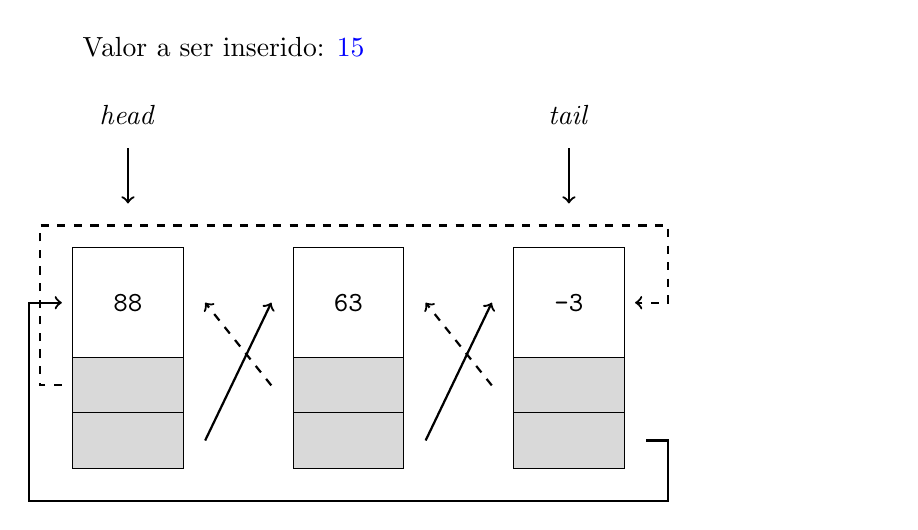
\begin{tikzpicture}[scale=1.4]
        \node[anchor=north west] at (0, 4) {Valor a ser inserido: \textcolor{blue}{15}};

        \node[anchor=center] at (0.5, 3.2) {\textit{head}};
        \draw[->,thick] (0.5, 2.9) -- (0.5, 2.4);

        \node[anchor=center] at (4.5, 3.2) {\textit{tail}};
        \draw[->,thick] (4.5, 2.9) -- (4.5, 2.4);

        \draw[opacity=0,->,thick] (7.2, 0.25) -- (7.4, 0.25) -- (7.4, -0.3) -- (-0.4, -0.3) -- (-0.4, 1.5) -- (-0.1, 1.5);
        \draw[opacity=0,->,thick,dashed] (-0.1, 0.75) -- (-0.3, 0.75) -- (-0.3, 2.2) -- (7.4, 2.2) -- (7.4, 1.5) -- (7.1, 1.5);

        \draw[opacity=1,->,thick] (5.2, 0.25) -- (5.4, 0.25) -- (5.4, -0.3) -- (-0.4, -0.3) -- (-0.4, 1.5) -- (-0.1, 1.5);
        \draw[opacity=1,->,thick,dashed] (-0.1, 0.75) -- (-0.3, 0.75) -- (-0.3, 2.2) -- (5.4, 2.2) -- (5.4, 1.5) -- (5.1, 1.5);

        \draw[fill=white] (0,1) rectangle (1,2);
        \draw[fill=gray!30] (0,0.5) rectangle (1,1);
        \draw[fill=gray!30] (0,0) rectangle (1,0.5);
        \node at (0.5,1.5) { \textcolor{black}{\texttt{88}}};

        \draw[->,thick] (1.2, 0.25) -- (1.8, 1.5);
        \draw[->,thick,dashed] (1.8, 0.75) -- (1.2, 1.5);

        \draw[fill=gray!30] (2,0) rectangle (3,0.5);
        \draw[fill=white] (2,1) rectangle (3,2);
        \draw[fill=gray!30] (2,0.5) rectangle (3,1);
        \draw[fill=gray!30] (2,0) rectangle (3,0.5);
        \node at (2.5,1.5) {\texttt{63}};

        \draw[->,thick] (3.2, 0.25) -- (3.8, 1.5);
        \draw[->,thick,dashed] (3.8, 0.75) -- (3.2, 1.5);

        \draw[fill=white] (4,1) rectangle (5,2);
        \draw[fill=gray!30] (4,0) rectangle (5,0.5);
        \draw[fill=gray!30] (4,0.5) rectangle (5,1);
        \node at (4.5,1.5) {\texttt{-3}};

%        \draw[->,thick] (5.2, 0.25) -- (5.8, 1.5);
%        \draw[->,thick,dashed] (5.8, 0.75) -- (5.2, 1.5);

        \draw[opacity=0,fill=white] (6,1) rectangle (7,2);
%        \draw[fill=gray!30] (6,0) rectangle (7,0.5);
%        \draw[fill=gray!30] (6,0.5) rectangle (7,1);
%        \node at (6.5,1.5) {\texttt{27}};

    \end{tikzpicture}

\end{frame}

\begin{frame}[fragile]{Visualização da inserção no final}

    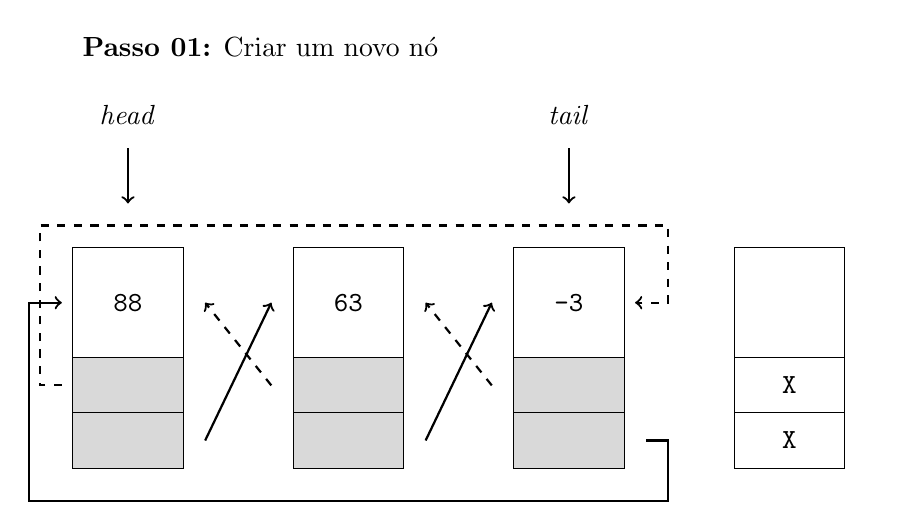
\begin{tikzpicture}[scale=1.4]
        \node[anchor=north west] at (0, 4) {\textbf{Passo 01:} Criar um novo nó};

        \node[anchor=center] at (0.5, 3.2) {\textit{head}};
        \draw[->,thick] (0.5, 2.9) -- (0.5, 2.4);

        \node[anchor=center] at (4.5, 3.2) {\textit{tail}};
        \draw[->,thick] (4.5, 2.9) -- (4.5, 2.4);

        \draw[opacity=0,->,thick] (7.2, 0.25) -- (7.4, 0.25) -- (7.4, -0.3) -- (-0.4, -0.3) -- (-0.4, 1.5) -- (-0.1, 1.5);
        \draw[opacity=0,->,thick,dashed] (-0.1, 0.75) -- (-0.3, 0.75) -- (-0.3, 2.2) -- (7.4, 2.2) -- (7.4, 1.5) -- (7.1, 1.5);

        \draw[opacity=1,->,thick] (5.2, 0.25) -- (5.4, 0.25) -- (5.4, -0.3) -- (-0.4, -0.3) -- (-0.4, 1.5) -- (-0.1, 1.5);
        \draw[opacity=1,->,thick,dashed] (-0.1, 0.75) -- (-0.3, 0.75) -- (-0.3, 2.2) -- (5.4, 2.2) -- (5.4, 1.5) -- (5.1, 1.5);

        \draw[fill=white] (0,1) rectangle (1,2);
        \draw[fill=gray!30] (0,0.5) rectangle (1,1);
        \draw[fill=gray!30] (0,0) rectangle (1,0.5);
        \node at (0.5,1.5) { \textcolor{black}{\texttt{88}}};

        \draw[->,thick] (1.2, 0.25) -- (1.8, 1.5);
        \draw[->,thick,dashed] (1.8, 0.75) -- (1.2, 1.5);

        \draw[fill=gray!30] (2,0) rectangle (3,0.5);
        \draw[fill=white] (2,1) rectangle (3,2);
        \draw[fill=gray!30] (2,0.5) rectangle (3,1);
        \draw[fill=gray!30] (2,0) rectangle (3,0.5);
        \node at (2.5,1.5) {\texttt{63}};

        \draw[->,thick] (3.2, 0.25) -- (3.8, 1.5);
        \draw[->,thick,dashed] (3.8, 0.75) -- (3.2, 1.5);

        \draw[fill=white] (4,1) rectangle (5,2);
        \draw[fill=gray!30] (4,0) rectangle (5,0.5);
        \draw[fill=gray!30] (4,0.5) rectangle (5,1);
        \node at (4.5,1.5) {\texttt{-3}};

%        \draw[->,thick] (5.2, 0.25) -- (5.8, 1.5);
%        \draw[->,thick,dashed] (5.8, 0.75) -- (5.2, 1.5);

        \draw[opacity=1,fill=white] (6,1) rectangle (7,2);
        \draw[fill=white!30] (6,0) rectangle (7,0.5);
        \draw[fill=white!30] (6,0.5) rectangle (7,1);
        \node at (6.5,1.5) {\texttt{}};
        \node at (6.5,0.75) {\textbf{\texttt{X}}};
        \node at (6.5,0.25) {\textbf{\texttt{X}}};

    \end{tikzpicture}

\end{frame}

\begin{frame}[fragile]{Visualização da inserção no final}

    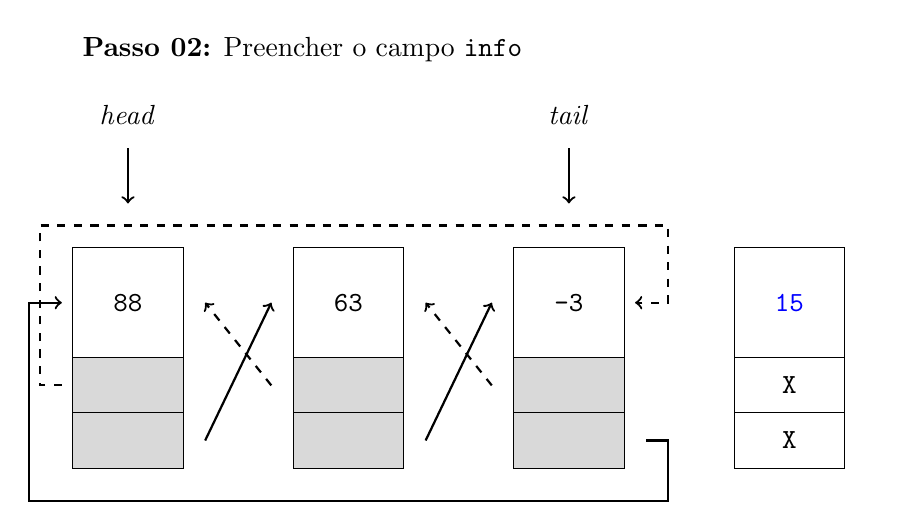
\begin{tikzpicture}[scale=1.4]
        \node[anchor=north west] at (0, 4) {\textbf{Passo 02:} Preencher o campo \texttt{info}};

        \node[anchor=center] at (0.5, 3.2) {\textit{head}};
        \draw[->,thick] (0.5, 2.9) -- (0.5, 2.4);

        \node[anchor=center] at (4.5, 3.2) {\textit{tail}};
        \draw[->,thick] (4.5, 2.9) -- (4.5, 2.4);

        \draw[opacity=0,->,thick] (7.2, 0.25) -- (7.4, 0.25) -- (7.4, -0.3) -- (-0.4, -0.3) -- (-0.4, 1.5) -- (-0.1, 1.5);
        \draw[opacity=0,->,thick,dashed] (-0.1, 0.75) -- (-0.3, 0.75) -- (-0.3, 2.2) -- (7.4, 2.2) -- (7.4, 1.5) -- (7.1, 1.5);

        \draw[opacity=1,->,thick] (5.2, 0.25) -- (5.4, 0.25) -- (5.4, -0.3) -- (-0.4, -0.3) -- (-0.4, 1.5) -- (-0.1, 1.5);
        \draw[opacity=1,->,thick,dashed] (-0.1, 0.75) -- (-0.3, 0.75) -- (-0.3, 2.2) -- (5.4, 2.2) -- (5.4, 1.5) -- (5.1, 1.5);

        \draw[fill=white] (0,1) rectangle (1,2);
        \draw[fill=gray!30] (0,0.5) rectangle (1,1);
        \draw[fill=gray!30] (0,0) rectangle (1,0.5);
        \node at (0.5,1.5) { \textcolor{black}{\texttt{88}}};

        \draw[->,thick] (1.2, 0.25) -- (1.8, 1.5);
        \draw[->,thick,dashed] (1.8, 0.75) -- (1.2, 1.5);

        \draw[fill=gray!30] (2,0) rectangle (3,0.5);
        \draw[fill=white] (2,1) rectangle (3,2);
        \draw[fill=gray!30] (2,0.5) rectangle (3,1);
        \draw[fill=gray!30] (2,0) rectangle (3,0.5);
        \node at (2.5,1.5) {\texttt{63}};

        \draw[->,thick] (3.2, 0.25) -- (3.8, 1.5);
        \draw[->,thick,dashed] (3.8, 0.75) -- (3.2, 1.5);

        \draw[fill=white] (4,1) rectangle (5,2);
        \draw[fill=gray!30] (4,0) rectangle (5,0.5);
        \draw[fill=gray!30] (4,0.5) rectangle (5,1);
        \node at (4.5,1.5) {\texttt{-3}};

%        \draw[->,thick] (5.2, 0.25) -- (5.8, 1.5);
%        \draw[->,thick,dashed] (5.8, 0.75) -- (5.2, 1.5);

        \draw[opacity=1,fill=white] (6,1) rectangle (7,2);
        \draw[fill=white!30] (6,0) rectangle (7,0.5);
        \draw[fill=white!30] (6,0.5) rectangle (7,1);
        \node at (6.5,1.5) {\textcolor{blue}{\texttt{15}}};
        \node at (6.5,0.75) {\textbf{\texttt{X}}};
        \node at (6.5,0.25) {\textbf{\texttt{X}}};

    \end{tikzpicture}

\end{frame}

\begin{frame}[fragile]{Visualização da inserção no final}

    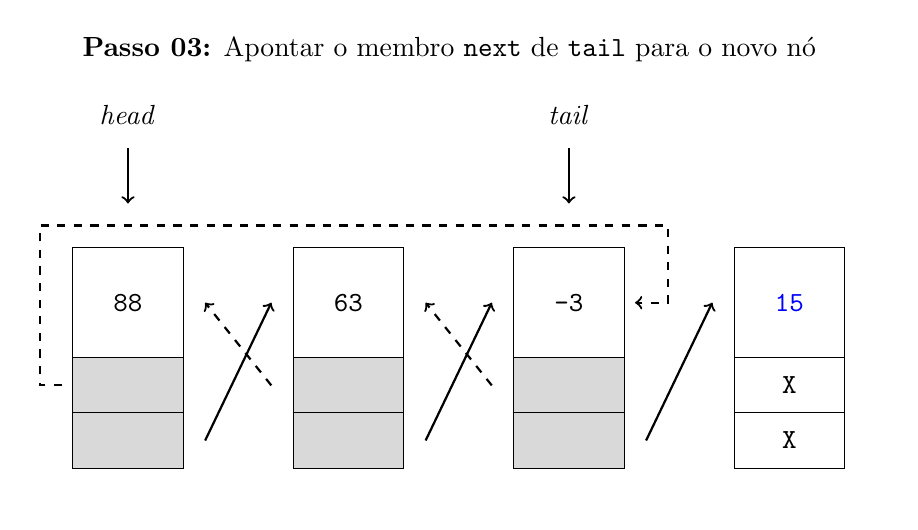
\begin{tikzpicture}[scale=1.4]
        \node[anchor=north west] at (0, 4) {\textbf{Passo 03:} Apontar o membro \texttt{next} de \texttt{tail} para o novo nó};

        \node[anchor=center] at (0.5, 3.2) {\textit{head}};
        \draw[->,thick] (0.5, 2.9) -- (0.5, 2.4);

        \node[anchor=center] at (4.5, 3.2) {\textit{tail}};
        \draw[->,thick] (4.5, 2.9) -- (4.5, 2.4);

        \draw[opacity=0,->,thick] (7.2, 0.25) -- (7.4, 0.25) -- (7.4, -0.3) -- (-0.4, -0.3) -- (-0.4, 1.5) -- (-0.1, 1.5);
        \draw[opacity=0,->,thick,dashed] (-0.1, 0.75) -- (-0.3, 0.75) -- (-0.3, 2.2) -- (7.4, 2.2) -- (7.4, 1.5) -- (7.1, 1.5);

        \draw[opacity=0,->,thick] (5.2, 0.25) -- (5.4, 0.25) -- (5.4, -0.3) -- (-0.4, -0.3) -- (-0.4, 1.5) -- (-0.1, 1.5);
        \draw[opacity=1,->,thick,dashed] (-0.1, 0.75) -- (-0.3, 0.75) -- (-0.3, 2.2) -- (5.4, 2.2) -- (5.4, 1.5) -- (5.1, 1.5);

        \draw[fill=white] (0,1) rectangle (1,2);
        \draw[fill=gray!30] (0,0.5) rectangle (1,1);
        \draw[fill=gray!30] (0,0) rectangle (1,0.5);
        \node at (0.5,1.5) { \textcolor{black}{\texttt{88}}};

        \draw[->,thick] (1.2, 0.25) -- (1.8, 1.5);
        \draw[->,thick,dashed] (1.8, 0.75) -- (1.2, 1.5);

        \draw[fill=gray!30] (2,0) rectangle (3,0.5);
        \draw[fill=white] (2,1) rectangle (3,2);
        \draw[fill=gray!30] (2,0.5) rectangle (3,1);
        \draw[fill=gray!30] (2,0) rectangle (3,0.5);
        \node at (2.5,1.5) {\texttt{63}};

        \draw[->,thick] (3.2, 0.25) -- (3.8, 1.5);
        \draw[->,thick,dashed] (3.8, 0.75) -- (3.2, 1.5);

        \draw[fill=white] (4,1) rectangle (5,2);
        \draw[fill=gray!30] (4,0) rectangle (5,0.5);
        \draw[fill=gray!30] (4,0.5) rectangle (5,1);
        \node at (4.5,1.5) {\texttt{-3}};

        \draw[->,thick] (5.2, 0.25) -- (5.8, 1.5);
%        \draw[->,thick,dashed] (5.8, 0.75) -- (5.2, 1.5);

        \draw[opacity=1,fill=white] (6,1) rectangle (7,2);
        \draw[fill=white!30] (6,0) rectangle (7,0.5);
        \draw[fill=white!30] (6,0.5) rectangle (7,1);
        \node at (6.5,1.5) {\textcolor{blue}{\texttt{15}}};
        \node at (6.5,0.75) {\textbf{\texttt{X}}};
        \node at (6.5,0.25) {\textbf{\texttt{X}}};

    \end{tikzpicture}

\end{frame}

\begin{frame}[fragile]{Visualização da inserção no final}

    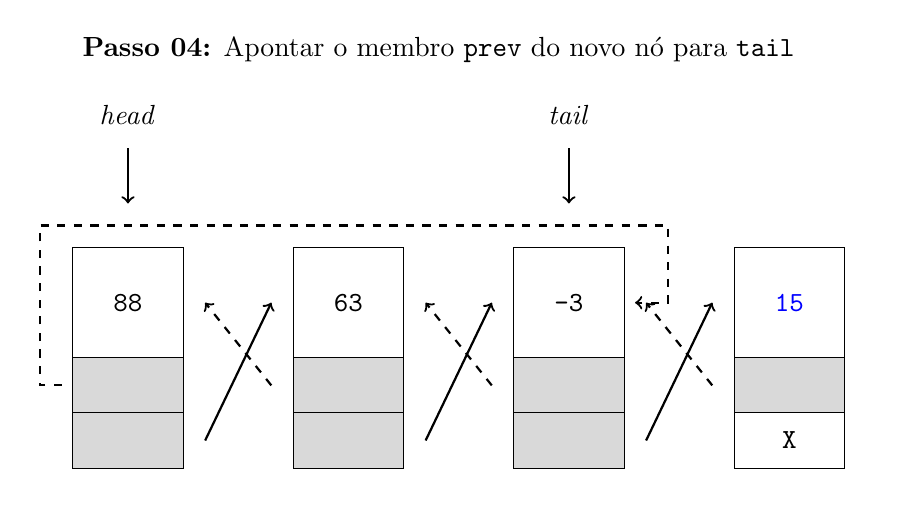
\begin{tikzpicture}[scale=1.4]
        \node[anchor=north west] at (0, 4) {\textbf{Passo 04:} Apontar o membro \texttt{prev} do novo nó para \texttt{tail}};

        \node[anchor=center] at (0.5, 3.2) {\textit{head}};
        \draw[->,thick] (0.5, 2.9) -- (0.5, 2.4);

        \node[anchor=center] at (4.5, 3.2) {\textit{tail}};
        \draw[->,thick] (4.5, 2.9) -- (4.5, 2.4);

        \draw[opacity=0,->,thick] (7.2, 0.25) -- (7.4, 0.25) -- (7.4, -0.3) -- (-0.4, -0.3) -- (-0.4, 1.5) -- (-0.1, 1.5);
        \draw[opacity=0,->,thick,dashed] (-0.1, 0.75) -- (-0.3, 0.75) -- (-0.3, 2.2) -- (7.4, 2.2) -- (7.4, 1.5) -- (7.1, 1.5);

        \draw[opacity=0,->,thick] (5.2, 0.25) -- (5.4, 0.25) -- (5.4, -0.3) -- (-0.4, -0.3) -- (-0.4, 1.5) -- (-0.1, 1.5);
        \draw[opacity=1,->,thick,dashed] (-0.1, 0.75) -- (-0.3, 0.75) -- (-0.3, 2.2) -- (5.4, 2.2) -- (5.4, 1.5) -- (5.1, 1.5);

        \draw[fill=white] (0,1) rectangle (1,2);
        \draw[fill=gray!30] (0,0.5) rectangle (1,1);
        \draw[fill=gray!30] (0,0) rectangle (1,0.5);
        \node at (0.5,1.5) { \textcolor{black}{\texttt{88}}};

        \draw[->,thick] (1.2, 0.25) -- (1.8, 1.5);
        \draw[->,thick,dashed] (1.8, 0.75) -- (1.2, 1.5);

        \draw[fill=gray!30] (2,0) rectangle (3,0.5);
        \draw[fill=white] (2,1) rectangle (3,2);
        \draw[fill=gray!30] (2,0.5) rectangle (3,1);
        \draw[fill=gray!30] (2,0) rectangle (3,0.5);
        \node at (2.5,1.5) {\texttt{63}};

        \draw[->,thick] (3.2, 0.25) -- (3.8, 1.5);
        \draw[->,thick,dashed] (3.8, 0.75) -- (3.2, 1.5);

        \draw[fill=white] (4,1) rectangle (5,2);
        \draw[fill=gray!30] (4,0) rectangle (5,0.5);
        \draw[fill=gray!30] (4,0.5) rectangle (5,1);
        \node at (4.5,1.5) {\texttt{-3}};

        \draw[->,thick] (5.2, 0.25) -- (5.8, 1.5);
        \draw[->,thick,dashed] (5.8, 0.75) -- (5.2, 1.5);

        \draw[opacity=1,fill=white] (6,1) rectangle (7,2);
        \draw[fill=white!30] (6,0) rectangle (7,0.5);
        \draw[fill=gray!30] (6,0.5) rectangle (7,1);
        \node at (6.5,1.5) {\textcolor{blue}{\texttt{15}}};
        \node at (6.5,0.25) {\textbf{\texttt{X}}};

    \end{tikzpicture}

\end{frame}

\begin{frame}[fragile]{Visualização da inserção no final}

    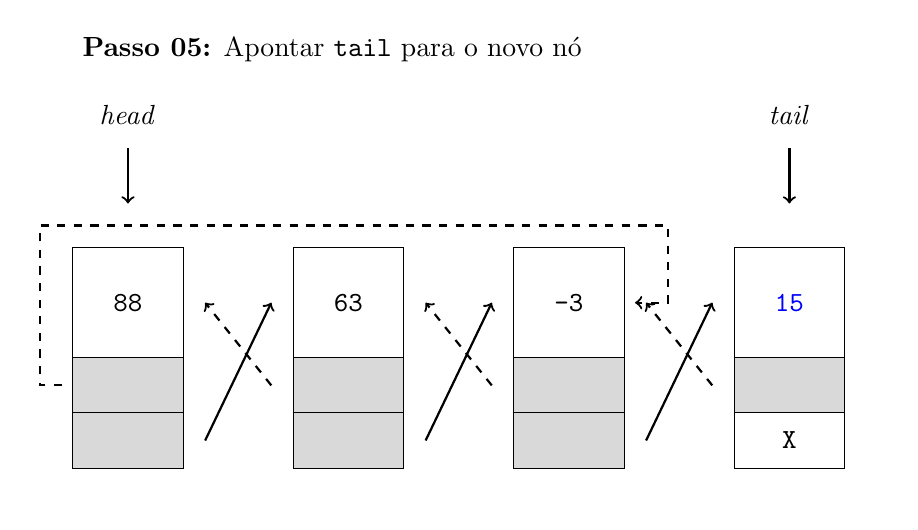
\begin{tikzpicture}[scale=1.4]
        \node[anchor=north west] at (0, 4) {\textbf{Passo 05:} Apontar \texttt{tail} para o novo nó };

        \node[anchor=center] at (0.5, 3.2) {\textit{head}};
        \draw[->,thick] (0.5, 2.9) -- (0.5, 2.4);

        \node[anchor=center] at (6.5, 3.2) {\textit{tail}};
        \draw[->,thick] (6.5, 2.9) -- (6.5, 2.4);

        \draw[opacity=0,->,thick] (7.2, 0.25) -- (7.4, 0.25) -- (7.4, -0.3) -- (-0.4, -0.3) -- (-0.4, 1.5) -- (-0.1, 1.5);
        \draw[opacity=0,->,thick,dashed] (-0.1, 0.75) -- (-0.3, 0.75) -- (-0.3, 2.2) -- (7.4, 2.2) -- (7.4, 1.5) -- (7.1, 1.5);

        \draw[opacity=0,->,thick] (5.2, 0.25) -- (5.4, 0.25) -- (5.4, -0.3) -- (-0.4, -0.3) -- (-0.4, 1.5) -- (-0.1, 1.5);
        \draw[opacity=1,->,thick,dashed] (-0.1, 0.75) -- (-0.3, 0.75) -- (-0.3, 2.2) -- (5.4, 2.2) -- (5.4, 1.5) -- (5.1, 1.5);

        \draw[fill=white] (0,1) rectangle (1,2);
        \draw[fill=gray!30] (0,0.5) rectangle (1,1);
        \draw[fill=gray!30] (0,0) rectangle (1,0.5);
        \node at (0.5,1.5) { \textcolor{black}{\texttt{88}}};

        \draw[->,thick] (1.2, 0.25) -- (1.8, 1.5);
        \draw[->,thick,dashed] (1.8, 0.75) -- (1.2, 1.5);

        \draw[fill=gray!30] (2,0) rectangle (3,0.5);
        \draw[fill=white] (2,1) rectangle (3,2);
        \draw[fill=gray!30] (2,0.5) rectangle (3,1);
        \draw[fill=gray!30] (2,0) rectangle (3,0.5);
        \node at (2.5,1.5) {\texttt{63}};

        \draw[->,thick] (3.2, 0.25) -- (3.8, 1.5);
        \draw[->,thick,dashed] (3.8, 0.75) -- (3.2, 1.5);

        \draw[fill=white] (4,1) rectangle (5,2);
        \draw[fill=gray!30] (4,0) rectangle (5,0.5);
        \draw[fill=gray!30] (4,0.5) rectangle (5,1);
        \node at (4.5,1.5) {\texttt{-3}};

        \draw[->,thick] (5.2, 0.25) -- (5.8, 1.5);
        \draw[->,thick,dashed] (5.8, 0.75) -- (5.2, 1.5);

        \draw[opacity=1,fill=white] (6,1) rectangle (7,2);
        \draw[fill=white!30] (6,0) rectangle (7,0.5);
        \draw[fill=gray!30] (6,0.5) rectangle (7,1);
        \node at (6.5,1.5) {\textcolor{blue}{\texttt{15}}};
        \node at (6.5,0.25) {\textbf{\texttt{X}}};

    \end{tikzpicture}

\end{frame}

\begin{frame}[fragile]{Visualização da inserção no final}

    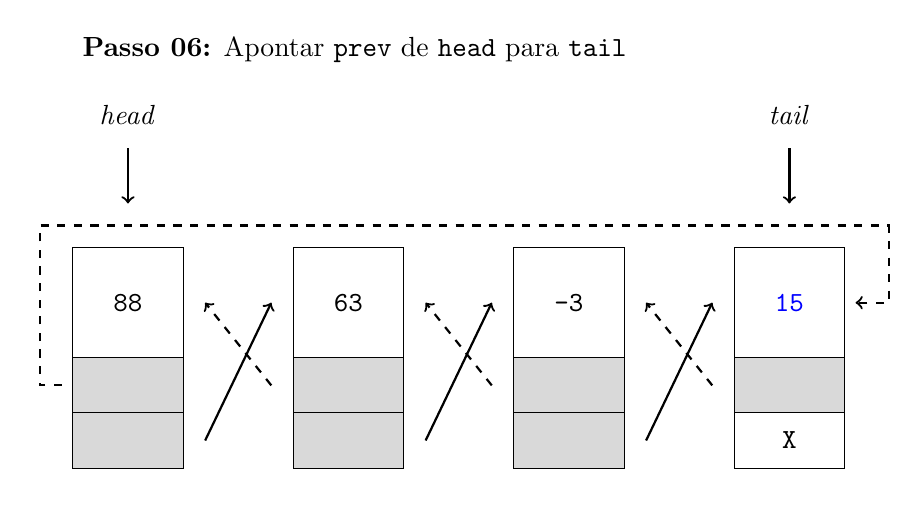
\begin{tikzpicture}[scale=1.4]
        \node[anchor=north west] at (0, 4) {\textbf{Passo 06:} Apontar \texttt{prev} de \texttt{head} para \texttt{tail} };

        \node[anchor=center] at (0.5, 3.2) {\textit{head}};
        \draw[->,thick] (0.5, 2.9) -- (0.5, 2.4);

        \node[anchor=center] at (6.5, 3.2) {\textit{tail}};
        \draw[->,thick] (6.5, 2.9) -- (6.5, 2.4);

        \draw[opacity=0,->,thick] (7.2, 0.25) -- (7.4, 0.25) -- (7.4, -0.3) -- (-0.4, -0.3) -- (-0.4, 1.5) -- (-0.1, 1.5);
        \draw[opacity=1,->,thick,dashed] (-0.1, 0.75) -- (-0.3, 0.75) -- (-0.3, 2.2) -- (7.4, 2.2) -- (7.4, 1.5) -- (7.1, 1.5);

        \draw[opacity=0,->,thick] (5.2, 0.25) -- (5.4, 0.25) -- (5.4, -0.3) -- (-0.4, -0.3) -- (-0.4, 1.5) -- (-0.1, 1.5);
        \draw[opacity=0,->,thick,dashed] (-0.1, 0.75) -- (-0.3, 0.75) -- (-0.3, 2.2) -- (5.4, 2.2) -- (5.4, 1.5) -- (5.1, 1.5);

        \draw[fill=white] (0,1) rectangle (1,2);
        \draw[fill=gray!30] (0,0.5) rectangle (1,1);
        \draw[fill=gray!30] (0,0) rectangle (1,0.5);
        \node at (0.5,1.5) { \textcolor{black}{\texttt{88}}};

        \draw[->,thick] (1.2, 0.25) -- (1.8, 1.5);
        \draw[->,thick,dashed] (1.8, 0.75) -- (1.2, 1.5);

        \draw[fill=gray!30] (2,0) rectangle (3,0.5);
        \draw[fill=white] (2,1) rectangle (3,2);
        \draw[fill=gray!30] (2,0.5) rectangle (3,1);
        \draw[fill=gray!30] (2,0) rectangle (3,0.5);
        \node at (2.5,1.5) {\texttt{63}};

        \draw[->,thick] (3.2, 0.25) -- (3.8, 1.5);
        \draw[->,thick,dashed] (3.8, 0.75) -- (3.2, 1.5);

        \draw[fill=white] (4,1) rectangle (5,2);
        \draw[fill=gray!30] (4,0) rectangle (5,0.5);
        \draw[fill=gray!30] (4,0.5) rectangle (5,1);
        \node at (4.5,1.5) {\texttt{-3}};

        \draw[->,thick] (5.2, 0.25) -- (5.8, 1.5);
        \draw[->,thick,dashed] (5.8, 0.75) -- (5.2, 1.5);

        \draw[opacity=1,fill=white] (6,1) rectangle (7,2);
        \draw[fill=white!30] (6,0) rectangle (7,0.5);
        \draw[fill=gray!30] (6,0.5) rectangle (7,1);
        \node at (6.5,1.5) {\textcolor{blue}{\texttt{15}}};
        \node at (6.5,0.25) {\textbf{\texttt{X}}};

    \end{tikzpicture}

\end{frame}

\begin{frame}[fragile]{Visualização da inserção no final}

    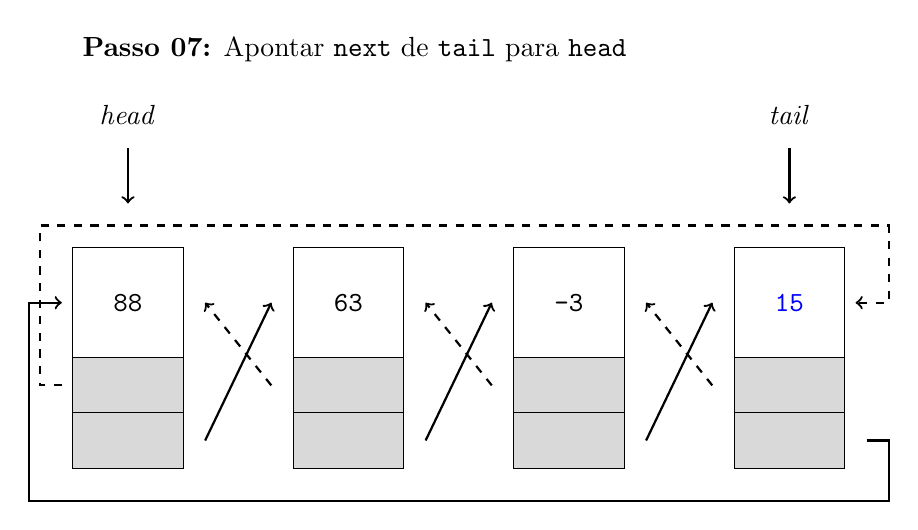
\begin{tikzpicture}[scale=1.4]
        \node[anchor=north west] at (0, 4) {\textbf{Passo 07:} Apontar \texttt{next} de \texttt{tail} para \texttt{head} };

        \node[anchor=center] at (0.5, 3.2) {\textit{head}};
        \draw[->,thick] (0.5, 2.9) -- (0.5, 2.4);

        \node[anchor=center] at (6.5, 3.2) {\textit{tail}};
        \draw[->,thick] (6.5, 2.9) -- (6.5, 2.4);

        \draw[opacity=1,->,thick] (7.2, 0.25) -- (7.4, 0.25) -- (7.4, -0.3) -- (-0.4, -0.3) -- (-0.4, 1.5) -- (-0.1, 1.5);
        \draw[opacity=1,->,thick,dashed] (-0.1, 0.75) -- (-0.3, 0.75) -- (-0.3, 2.2) -- (7.4, 2.2) -- (7.4, 1.5) -- (7.1, 1.5);

        \draw[opacity=0,->,thick] (5.2, 0.25) -- (5.4, 0.25) -- (5.4, -0.3) -- (-0.4, -0.3) -- (-0.4, 1.5) -- (-0.1, 1.5);
        \draw[opacity=0,->,thick,dashed] (-0.1, 0.75) -- (-0.3, 0.75) -- (-0.3, 2.2) -- (5.4, 2.2) -- (5.4, 1.5) -- (5.1, 1.5);

        \draw[fill=white] (0,1) rectangle (1,2);
        \draw[fill=gray!30] (0,0.5) rectangle (1,1);
        \draw[fill=gray!30] (0,0) rectangle (1,0.5);
        \node at (0.5,1.5) { \textcolor{black}{\texttt{88}}};

        \draw[->,thick] (1.2, 0.25) -- (1.8, 1.5);
        \draw[->,thick,dashed] (1.8, 0.75) -- (1.2, 1.5);

        \draw[fill=gray!30] (2,0) rectangle (3,0.5);
        \draw[fill=white] (2,1) rectangle (3,2);
        \draw[fill=gray!30] (2,0.5) rectangle (3,1);
        \draw[fill=gray!30] (2,0) rectangle (3,0.5);
        \node at (2.5,1.5) {\texttt{63}};

        \draw[->,thick] (3.2, 0.25) -- (3.8, 1.5);
        \draw[->,thick,dashed] (3.8, 0.75) -- (3.2, 1.5);

        \draw[fill=white] (4,1) rectangle (5,2);
        \draw[fill=gray!30] (4,0) rectangle (5,0.5);
        \draw[fill=gray!30] (4,0.5) rectangle (5,1);
        \node at (4.5,1.5) {\texttt{-3}};

        \draw[->,thick] (5.2, 0.25) -- (5.8, 1.5);
        \draw[->,thick,dashed] (5.8, 0.75) -- (5.2, 1.5);

        \draw[opacity=1,fill=white] (6,1) rectangle (7,2);
        \draw[fill=gray!30] (6,0) rectangle (7,0.5);
        \draw[fill=gray!30] (6,0.5) rectangle (7,1);
        \node at (6.5,1.5) {\textcolor{blue}{\texttt{15}}};

    \end{tikzpicture}

\end{frame}

\begin{frame}[fragile]{Implementação da inserção no final}
    \inputsnippet{c++}{142}{153}{circular_list.h}
\end{frame}

\begin{frame}[fragile]{Inserção em posição arbitrária}

    \begin{itemize}
        \item A inserção em posição arbitrária tem complexidade $O(N)$, onde $N$ é o número
            de elementos da lista, ou $O(1)$, caso o ponteiro para a posição onde o elemento
            será inserido seja conhecido

        \item Observe que, no caso dos vetores, mesmo que a posição de inserção seja conhecida,
            a complexidade permanece sendo $O(N)$

        \item É preciso ajustar adequadamente os membros \code{c}{prev} e \code{c}{next} do
            novo nó, de seu antecessor e de seu sucessor, caso existam

        \item Também é preciso ter cuidado com os ponteiros \code{c}{head} e \code{c}{tail}

        \item Há vários \textit{corner cases}:
            \begin{enumerate}
                \item Lista vazia
                \item Apenas um elemento na lista
                \item Inserção na primeira posição
                \item Posição de inserção inválida
            \end{enumerate}

    \end{itemize}

\end{frame}
